\documentclass[acmtog]{acmart}
\usepackage{graphicx}
\usepackage{subfigure}
\usepackage{natbib}
\usepackage{listings}
\usepackage{bm}
\usepackage{amsmath}

\definecolor{blve}{rgb}{0.3372549 , 0.61176471, 0.83921569}
\definecolor{gr33n}{rgb}{0.29019608, 0.7372549, 0.64705882}
\makeatletter
\lst@InstallKeywords k{class}{classstyle}\slshape{classstyle}{}ld
\makeatother
\lstset{language=C++,
	basicstyle=\ttfamily,
	keywordstyle=\color{blve}\ttfamily,
	stringstyle=\color{red}\ttfamily,
	commentstyle=\color{magenta}\ttfamily,
	morecomment=[l][\color{magenta}]{\#},
	classstyle = \bfseries\color{gr33n}, 
	tabsize=2
}
\lstset{basicstyle=\ttfamily}

% Title portion
\title{Assignment 3: {Ray Tracing Basics}} 

\author{Name:\quad Tian Haoyuan  \\ student number:\  2020533013
\\email:\quad tianhy@shanghaitech.edu.cn}

% Document starts
\begin{document}
\maketitle

\vspace*{2 ex}

\section{Introduction}
This project requires us to implement ray tracing in a scene to render the scene. Objects taking in consideration are geometries, the light, the camera, and also materials of geometries, and textures of materials. The core part of the project to me is the render() function in integrator.cpp, as well as intersect() function of each object.

Works that have been done are as follows.
\begin{itemize}
	\item Task1 generate rays from camera has been done.
	\item Task2 ray geometry intersection has been done.
	\item Task3 Phong lighting at intersection has been done.
	\item Task4 light ray sampling for soft shadow has been done.
	\item Task5 anti-aliasing by super-resolution has been done.
	\item Bonus1 texture mapping has been done.
	\item Bonus2 normal texture has been done.
	\item Bonus3 texture filtering using mip-map has been done.
	\item Bonus4 advanced anti-aliasing has been done.
\end{itemize}

\section{Implementation Details}
\subsection{Task1 generate rays from camera}
In camera.cpp, I implement lookAt() function of camera object, which defines the three vector of a camera.\\
Considering generating a ray from a camera, given dx,dy as the point on the image(focal), I first convert dx,dy to [-1,1), then determine the scale on both two coordinates, then I naturally obtain the displacement of the point from the middle point of the image as (0,0), which can also be determined by vector forward of the camera scaled be focal length.
Then I add two vector, displacements scaled respectively be up and right, to the middle point. Finally we have the vector from camera to the point, as the direction of the ray.

\subsection{Task2 ray geometry intersection}
Considering the process of rendering, intersections are called in the whole scene. The interseciton function of a scene may check intersecitons of light or geometries within the scene. The light, e.g. a square light, also has a geometry attribute to do intersecitons.\\
There are three geometries in the must part of this project, as well as the number of intersecitons to be implemented.\\
First comes the interseciton of triangle, given the ray and the triangle. I can naturally calculate the interseciton point of the ray and the triangle plane. Then I can determine whether the point locates inside the range of the triangle, by checking the coefficients of the triangle vertices. The second is the rectangle, after I get the point on the plane of the rectangle, I can simply know whether the point is inside the rectangle by checking the rectangle size.
And interseciton of ellipsode can be determined by M = TRS.\\
In the interseciton, we have to record information in the Object interaction, e.g. the interseciton position, the interseciton type, the distance from the camera to the interseciton, the normal and the Phong lighting model.
\subsection{Task3 Phong lighting at intersection}
In the process of rendering, after we get the interaction from the interseciton from an object to light, we have to render the object using Phong lighting model, which is kept in the interaction.\\
The process of Phong lighting is basically the same as what we have done in previous projects, using opengl with fragment shader. In this situation, we can obtain the ambient from the light easily, and the diffuse is also readily avilable since normal is just kept in the interaction, and light direction is an input.
However the reflect in fragment shader we used should be implementated by myself, then we can get the specular and add all of them together.
\subsection{Task4 light ray sampling for soft shadow}
Since it is a square light in the scene instead of a spot light, we have to sample some light samples when doing ray tracing. Considering the situation that it is a spot light in the scene, the shadows of all objects should be sharp, and we may make it soft by adding numbers of light samples, i.e. numbers of spot lights, then for each sample point in each pixel, taking the average of all light sample radiance, simulating the situation of the square light.
\subsection{Task5 anti-aliasing by super-resolution}
The image may look so rough till now, since we only sample each pixel once or several times, the lines and surfaces in the image may seem discrete rather than continuous, thus making it not real.\\
The point is to sample more points in each pixel. First I take samples in each pixel uniformally.
\begin{figure}[h]
	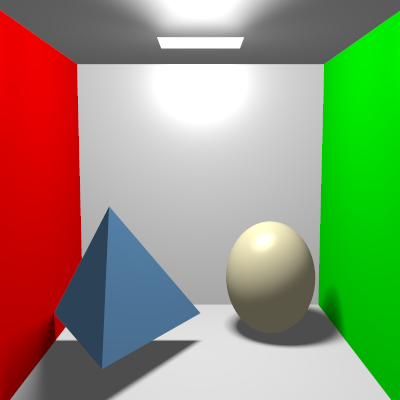
\includegraphics[width=4.5cm,height=4.5cm]{pp25_uniform.png}
	\caption{pp25\_uniform}
\end{figure}
in which I take 25 samples in each pixel, comparing to the origin that I take 4 samples per pixel:\\
\begin{figure}[h]
	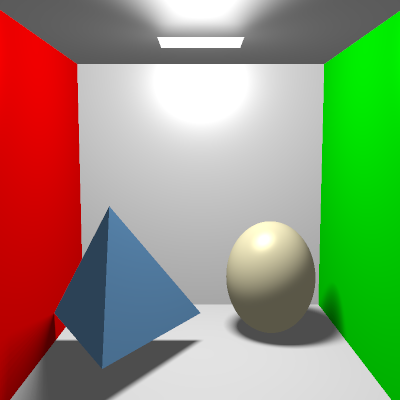
\includegraphics[width=4.5cm,height=4.5cm]{pp4_uniform.png}
	\caption{pp4\_uniform}
\end{figure}

And I also ramdomly generate 25 points within a pixel to sample, here is the result of 25 randomly generated samples per pixel.
\begin{figure}[h]
	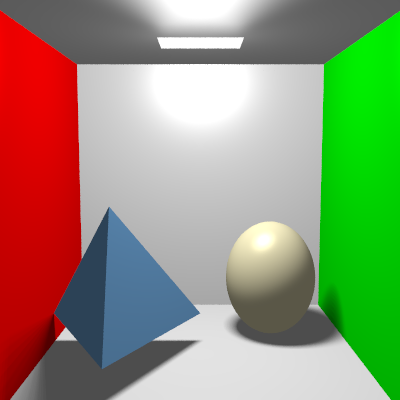
\includegraphics[width=4.5cm,height=4.5cm]{pp25_random.png}
	\caption{pp25\_random}
\end{figure}

This method performs well on curves such as on the ellipsode, and lines that are orthognal to the camera direction. Those excepted lines, for example the edge of the square light looks a little bit rough. This methos may converge when the sample per pixel get larger.\\
Both can pass the text on github.
\subsection{Bonus1 texture mapping}
Before this task, all materials of geometries in the scene are pure color materials. We should implement texture material TextureMat in material.cpp and the Texture object as well.\\
A material may have several textures, one is the outlook stored in text\_diff, and others are normal texture and displacement texture, that help rendering. For simplicity I keep an enumerate type in Material that record the material type, whether it is colormaterial or texture material, and keep those three texture in class material for after use. The point is that, when we evaluate from a material, we do not simply get the radiance directly like before, instead we should get the radiance from the texture diff of the material.\\
Thus keeping uv in interaction could be useful. uv is vector2f, both components range from 0 to 1. We can map uv between different size geometries and texture data.\\
Simply get the data from the texture is not enough, which could cause aliasing. When evaluating with a given uv on a material, or a texture. It should be better to perform interpolation on it, e.g. I do bilinear interpolation when evaluating. The idea of bilinear interpolation is trivial, as well as it's Implementation.
\subsection{Bonus2 normal texture}
Before applying normal texture to the texture material, the normal of the material is still the same as the normal of a rectangle. The light effect of rendering still resembles the rectangle.\\
I implement it in geometry intersecitons, especially rectangle. When doing interseciton, if the geometry is a texture, it should do interpolation to evaluate the point, and also if it has a normal texture text\_norm, then I should locate the correspond normal in normal texture by uv of the interaction. And keep it in the interaction instead of the rectangle normal.
\begin{figure}[h]
	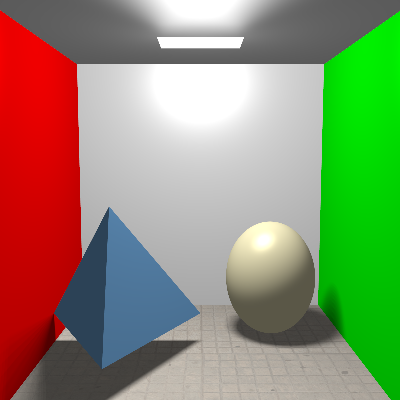
\includegraphics[width=4.5cm,height=4.5cm]{texture.png}
	\caption{texture with normal}
\end{figure}\\
It is slightly different from the former one that uses the rectangle normal. But it could definitely looks better if we implement displacement texture on that as well.
\subsection{Bonus3 texture filtering using mip-map}
Considering mipmap, first we should have several levels of data of the texture, so that each pixel can choose from when evaluating.\\
I generate levels of data when loading text\_diff, by averaging four close points in last level. Also I implement another geometry class named Ground, and specially implement its intersection, and also I implement a Material class named GoundMat, override the evaluate function.
Then we have fine tools to deal with the grid.\\
Without mipmap, the grid looks like this:
\begin{figure}[h]
	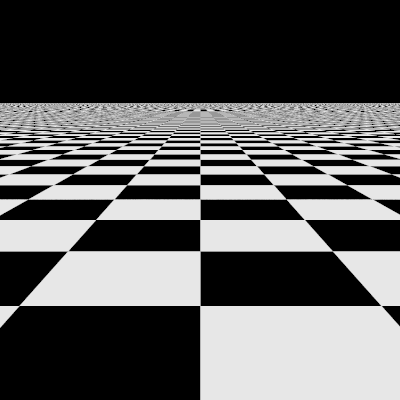
\includegraphics[width=4.5cm,height=4.5cm]{super_resolution_uniform.png}
	\caption{grid without mipmap, uniformally sampled}
\end{figure}\\
The point of mipmap is how to determine its level when evaluating. I took an approximation that, I can get the distance from the camera to the pixel, as well as the distance from camera to the interaction position,
and this is just the ratio of the cut and the pixel distance, where the cut is parallel with the image, and it should have an intersection angle, whose cosine is close to interaction.normal dot camera ray direction.
The result is like this,
\begin{figure}[h]
	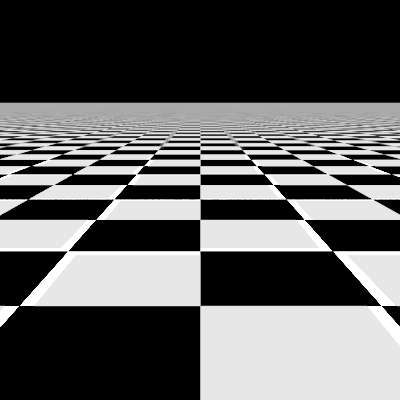
\includegraphics[width=4.5cm,height=4.5cm]{mipmap.png}
	\caption{grid with mipmap}
\end{figure}\\
\subsection{Bonus4 advanced anti-aliasing}
I implement rotated grid sampling.
I generate samples in a pixel uniformally, and then left multiply all vector3f by a rotate matrix2f,
$$\begin{bmatrix}
	\cos(\theta)&-\sin(\theta)\\
	\sin(\theta)&\cos(\theta)\\
\end{bmatrix},$$
taking the $\theta$ as $26.6$ degree.\\
This is the result of rotated grid in the original scene.
\begin{figure}[h]
	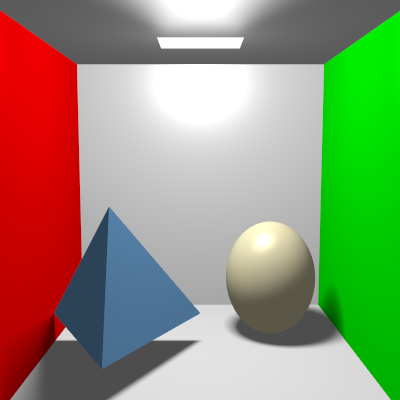
\includegraphics[width=4.5cm,height=4.5cm]{pp25_rotate.png}
	\caption{pp25\_rotate}
\end{figure}\\
And the following is the rotated grid sampling tested on grid.
\begin{figure}[h]
	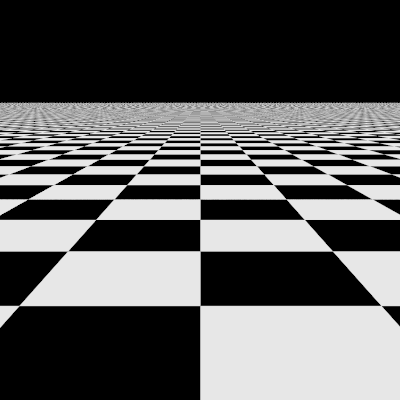
\includegraphics[width=4.5cm,height=4.5cm]{ground_rotate.png}
	\caption{grid rotatedly sampled}
\end{figure}\\
It is obvious that the pixels mapping to farther grid look better then that uniformally sampled. (comparing fig.8 to fig.5).
\section{Results}
% pictures should be in

\end{document}
